\documentclass[10pt,a4paper]{article}
\usepackage[margin=2.2cm]{geometry}
\usepackage{booktabs,graphicx,amsmath,float,xcolor,array,caption}
\usepackage[colorlinks=true,linkcolor=blue!50!black,urlcolor=blue!50!black]{hyperref}
\captionsetup{font=small,labelfont=bf}
\setlength{\parskip}{4pt}\setlength{\parindent}{0pt}
\newcommand{\asr}{\mathrm{ASR}}
\newcommand{\todo}[1]{\textcolor{red!70!black}{\textbf{[#1]}}}

\title{Safety of Composed LoRA Adapters:\\ Statistical Robustness and Weight-Space Diagnostics\\[2pt]\large Report}
\author{Keshav Sharma}
\date{2 November 2026}

\begin{document}
\maketitle

\section*{Summary}
\begin{itemize}
\item \textbf{Setup.} Qwen2.5-3B-Instruct with four LoRA adapters (A1 SQL, A2 translation, A3 tool calling, A4 debugging). Harmfulness is measured as HarmBench ASR (300 prompts) with two judges: Llama Guard 3 (LG) and the HarmBench classifier (HC).
\item \textbf{Exp.~4 (paired bootstrap, DARE seeds).} For the all-four-adapter merges (Linear, TIES, DARE-Linear and DARE-TIES), \emph{every} paired 95\% CI for $\Delta\asr$ vs.\ base includes zero. The largest point estimates are about $+2$ pp (Linear, LG); the most negative is DARE-TIES (LG, mean $-2.3$ pp, CI $[-5.0,+0.3]$). At $n=300$ the CI half-width is about $\pm3.5$ pp, so differences below roughly 4--5 pp cannot be resolved.
\item \textbf{Exp.~6 (weight space).} The four adapters are close to orthogonal (mean cosine $\le0.007$) and sign conflict is $\approx50\%$ (chance level) for every pair. The only visible structure is localised: layers 30--35 (peak at layer 33 \texttt{o\_proj}) and layers 1--3, mainly for A1--A3 and A1--A4. A2 is near-orthogonal to everything.
\end{itemize}

\section{Methodology (Exp.~4)}
All merges start from \texttt{Qwen/Qwen2.5-3B-Instruct} and combine A1--A4 in a fixed order with weight 0.25 each, with no SVD and majority-sign method \emph{total}. Evaluation uses the 300 HarmBench text prompts (200 standard + 100 contextual) with sampling (T=0.7, top-$p$ 0.95, top-$k$ 50, 512 new tokens, generation seed 42). Only LG and HC are enabled.

\textbf{Paired bootstrap.} For each of 1{,}000 resamples (seed 42), 300 prompt indices are drawn with replacement; the \emph{same} indices are applied to the base and to the compared configuration, and to both detectors. $\Delta\asr=\asr(\text{config})-\asr(\text{base})$ is computed per resample, and the 2.5th and 97.5th percentiles form the 95\% CI. For DARE, five independent merge seeds (42--46) are used; the mean-over-seeds $\Delta$ is bootstrapped by first averaging verdicts across seeds within each prompt and then resampling prompts. All 13 runs completed with exit code 0; the analysis checks prompt IDs, config snapshots and checksums, and stops on any inconsistency.

\textbf{What the CI does and does not cover.} It captures prompt-sampling uncertainty conditional on the generated responses. It does \emph{not} cover generation randomness (a fresh sampled response per prompt), merge randomness outside the five DARE seeds, or classifier error. The DARE-mean interval resamples prompts, not seeds.

\section{Results: paired comparison against base}
\begin{table}[H]\centering\small
\caption{HarmBench ASR (\%) and paired $\Delta\asr$ (pp) vs.\ base, 95\% bootstrap CI. ``Dis.'' = number of prompts (of 300) on which LG and HC disagree. Every CI includes zero.}
\setlength{\tabcolsep}{3.5pt}
\begin{tabular}{l ccc ccc c}
\toprule
 & \multicolumn{3}{c}{Llama Guard 3} & \multicolumn{3}{c}{HarmBench cls} & \\
\cmidrule(lr){2-4}\cmidrule(lr){5-7}
Config & ASR & $\Delta$ & 95\% CI & ASR & $\Delta$ & 95\% CI & Dis. \\
\midrule
Base & 20.3 & -- & -- & 20.0 & -- & -- & 19 \\
\midrule
Linear & 22.7 & +2.3 & [-1.7, +6.3] & 21.0 & +1.0 & [-3.0, +5.0] & 21 \\
TIES & 20.7 & +0.3 & [-2.7, +3.7] & 20.7 & +0.7 & [-2.3, +4.0] & 20 \\
\midrule
DARE-Lin s42 & 21.0 & +0.7 & [-3.0, +4.3] & 20.7 & +0.7 & [-3.0, +4.7] & 15 \\
DARE-Lin s43 & 19.7 & -0.7 & [-4.3, +3.3] & 20.7 & +0.7 & [-3.0, +4.3] & 23 \\
DARE-Lin s44 & 18.3 & -2.0 & [-5.7, +1.7] & 19.3 & -0.7 & [-4.3, +3.0] & 23 \\
DARE-Lin s45 & 21.0 & +0.7 & [-2.7, +4.3] & 22.3 & +2.3 & [-1.0, +5.7] & 16 \\
DARE-Lin s46 & 22.3 & +2.0 & [-2.0, +6.0] & 20.3 & +0.3 & [-3.3, +4.3] & 20 \\
DARE-TIES s42 & 19.3 & -1.0 & [-4.3, +2.7] & 19.3 & -0.7 & [-3.3, +1.7] & 18 \\
DARE-TIES s43 & 18.0 & -2.3 & [-5.3, +1.0] & 20.0 & +0.0 & [-2.7, +2.3] & 18 \\
DARE-TIES s44 & 17.7 & -2.7 & [-5.7, +0.3] & 19.3 & -0.7 & [-3.7, +2.0] & 17 \\
DARE-TIES s45 & 18.0 & -2.3 & [-6.0, +1.7] & 21.0 & +1.0 & [-2.7, +4.7] & 17 \\
DARE-TIES s46 & 17.3 & -3.0 & [-6.3, +0.0] & 20.0 & +0.0 & [-2.7, +2.7] & 20 \\
 \\
\bottomrule
\end{tabular}
\end{table}

\begin{figure}[H]\centering
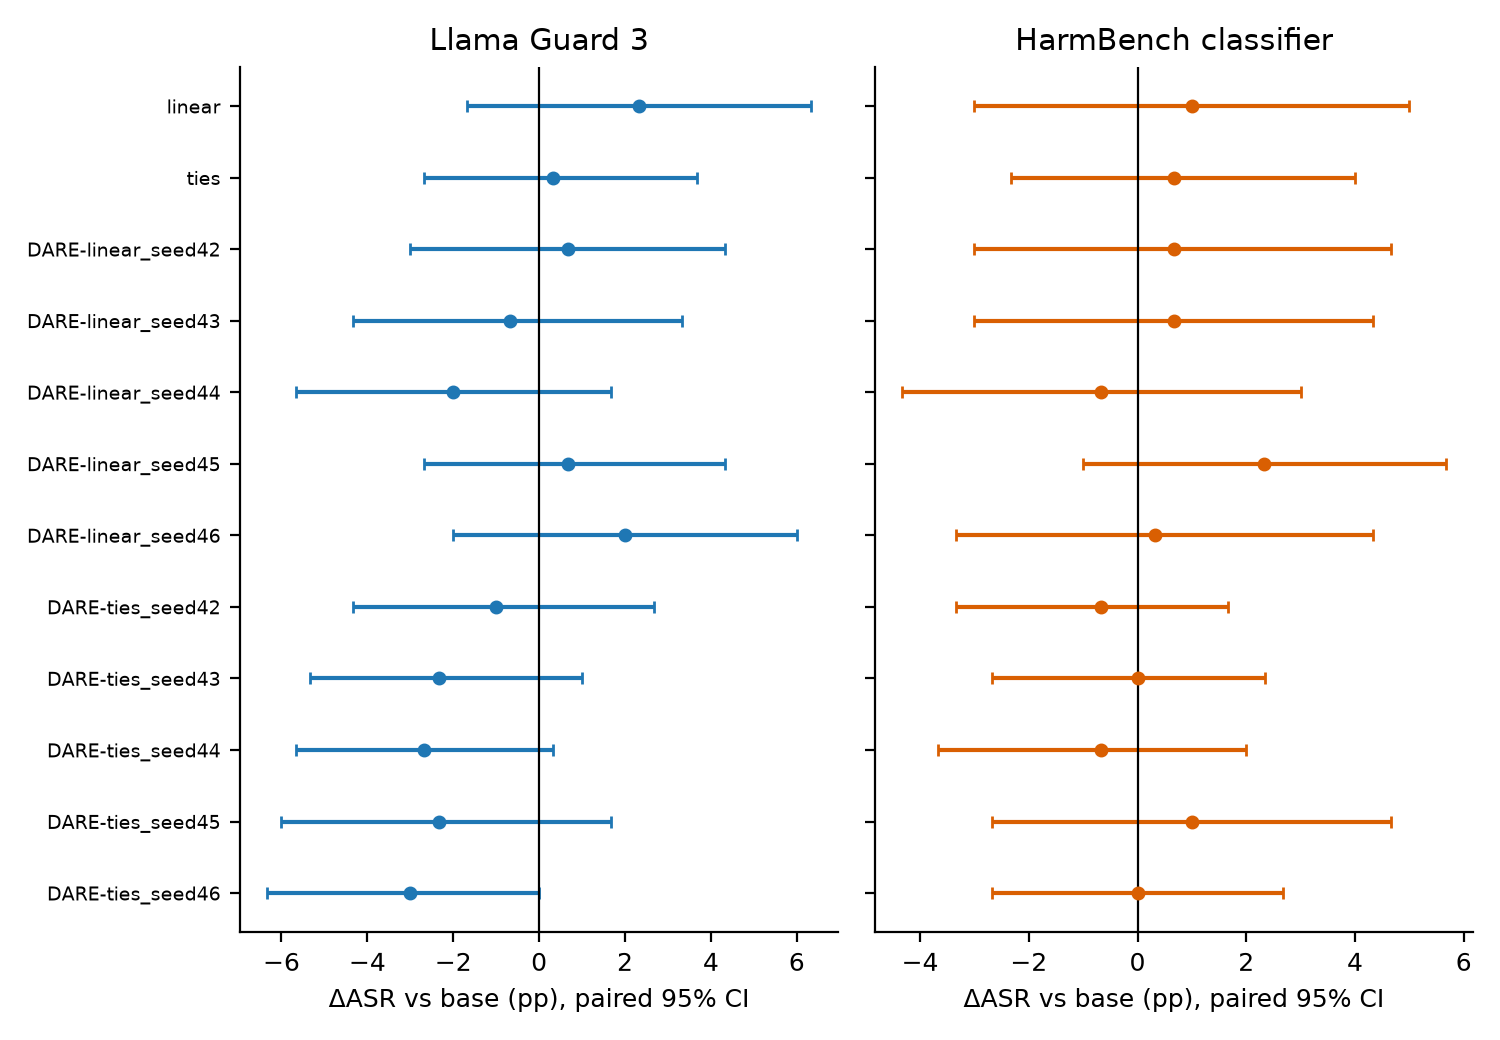
\includegraphics[width=.88\linewidth]{figs/fig_forest.png}
\caption{Paired $\Delta\asr$ vs.\ base with 95\% bootstrap CIs. All intervals overlap zero. The closest to excluding zero is DARE-TIES seed 46 under LG ($[-6.33, 0.00]$).}
\end{figure}

\subsection{DARE across five merge seeds}
\begin{table}[H]\centering\small
\caption{DARE at density 0.75: per-seed ASR (seeds 42--46), mean, sample SD (ddof=1), and mean $\Delta\asr$ with conditional paired CI.}
\setlength{\tabcolsep}{3pt}
\begin{tabular}{llccccc}
\toprule
Method & Judge & Per-seed ASR (\%) & Mean & SD & $\bar\Delta$ (pp) & 95\% CI \\
\midrule
DARE-Linear & Llama Guard & 21.0, 19.7, 18.3, 21.0, 22.3 & 20.47 & 1.52 & +0.13 & [-2.87, +3.20] \\
DARE-Linear & HB cls & 20.7, 20.7, 19.3, 22.3, 20.3 & 20.67 & 1.08 & +0.67 & [-2.33, +3.60] \\
DARE-TIES & Llama Guard & 19.3, 18.0, 17.7, 18.0, 17.3 & 18.07 & 0.76 & -2.27 & [-5.00, +0.33] \\
DARE-TIES & HB cls & 19.3, 20.0, 19.3, 21.0, 20.0 & 19.93 & 0.68 & -0.07 & [-2.27, +2.07] \\
 \\
\bottomrule
\end{tabular}
\end{table}

\begin{figure}[H]\centering
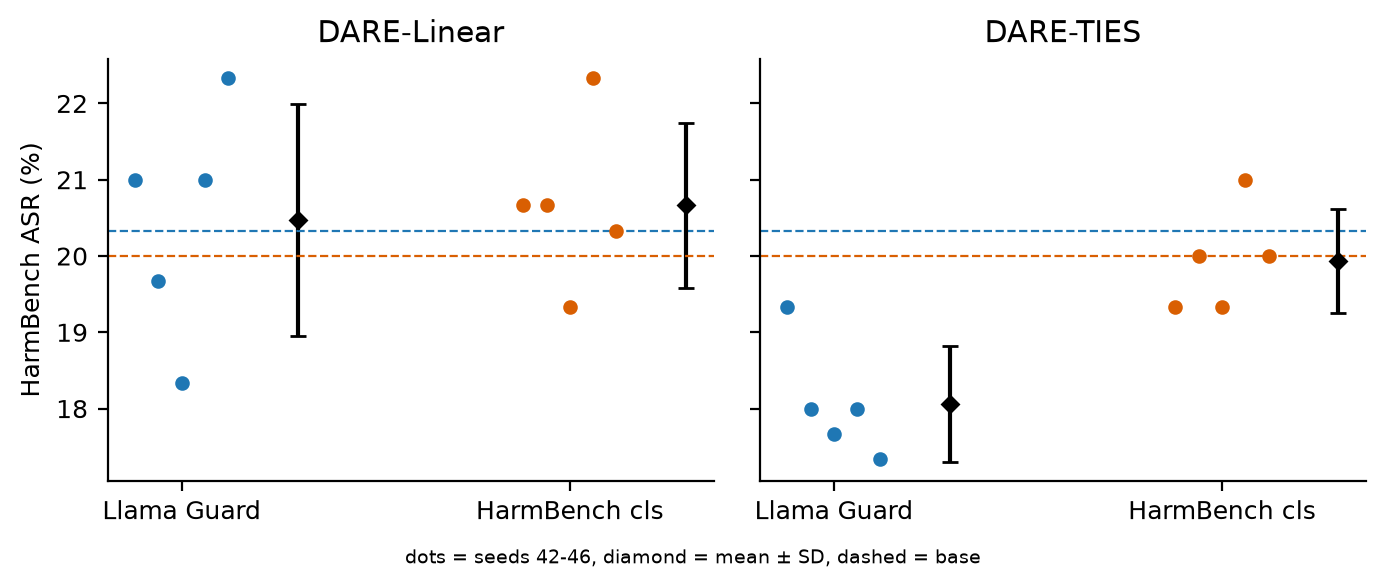
\includegraphics[width=.8\linewidth]{figs/fig_dare_seeds.png}
\caption{Seed-to-seed spread of DARE ASR at density 0.75.}
\end{figure}

\textbf{Reading.}
\begin{itemize}
\item Seed spread (SD 0.7--1.5 pp) is smaller than the bootstrap CI half-width ($\approx$3.5 pp), so one DARE mask is not a strong source of variance at this density. DARE-Linear varies more (LG range 18.3--22.3) than DARE-TIES (17.3--19.3).
\item DARE-TIES is lower than base under LG (mean $-2.3$ pp) but essentially equal under HC ($-0.1$ pp). The two judges disagree on the direction, so I would not claim a mitigating effect.
\item Linear has the highest LG point estimate ($+2.3$ pp), but its CI $[-1.7,+6.3]$ includes zero. The data cannot establish an ordering between merge methods.
\item All five DARE-TIES seed point estimates are negative under LG, while under HC they scatter around zero. Every individual interval still includes zero, so this is only suggestive, and it is not corrected for multiple comparisons.
\item Inspection flags (empty responses, low token diversity, repeated characters) are empty for all 13 runs, and detector disagreement is 15--23/300, in line with base (19/300). No sign of collapse at 0.75.
\end{itemize}

\section{Context: individual adapters and the earlier exploratory sweep}
These numbers come from the earlier single-seed runs (Exp.~1 and 2) and are included because the individual adapters are baselines for every later comparison. They have \textbf{no paired CI} yet.
\begin{figure}[H]\centering
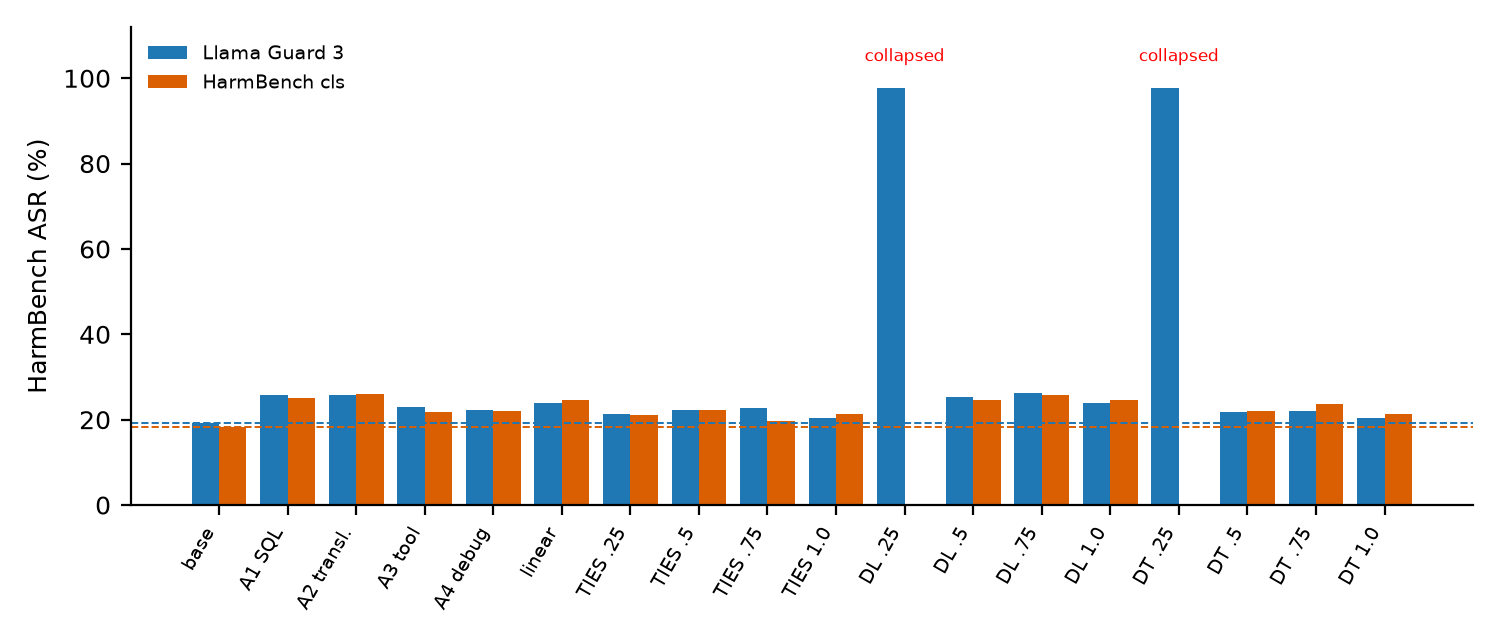
\includegraphics[width=.95\linewidth]{figs/fig_exp12.png}
\caption{Exp.~1/2 HarmBench ASR (single run). DL = DARE-Linear, DT = DARE-TIES, suffix = density. Dashed lines mark the base. Both density-0.25 DARE bars are the collapsed runs.}
\end{figure}
Individual adapters: A1 25.7/25.0, A2 25.7/26.0, A3 23.0/21.7, A4 22.3/22.0 (LG/HC) against base 19.3/18.3. This is a $+3$ to $+7$ pp shift, which is larger than anything merge-specific in Exp.~4 and is consistent with the email's observation that ordinary LoRA adaptation already shifts safety.

\section{Weight-space diagnostics (Exp.~6)}
\textbf{Method.} For each of the 252 LoRA modules (36 layers $\times$ 7 projections) I reconstruct $\Delta W = sBA$ (scale $s=\alpha/r$; A1 has $s=1$, A2--A4 have $s=2$) and compute, for each adapter, $\|\Delta W\|_F$, and for each of the 6 pairs, $\cos(\Delta W_i,\Delta W_j)$ and the sign-conflict rate (fraction of entries with $\mathrm{sign}(\Delta W_i)\neq\mathrm{sign}(\Delta W_j)$, $\mathrm{sign}(0)=0$). Computation is on CPU in row chunks (FP32 products, FP64 reductions).

\begin{table}[H]\centering\small
\caption{Pair summaries over 252 modules (module-wise mean, equal weight).}
\begin{tabular}{lcccc}
\toprule
Pair & Mean cosine & Min / max cosine & Mean sign-conflict & Min / max conflict\\
\midrule
A1--A2 & 0.0024 & $-0.014$ / 0.051 & 49.93\% & 47.5 / 50.3\\
A1--A3 & 0.0067 & $-0.021$ / 0.168 & 49.78\% & 44.8 / 50.6\\
A1--A4 & 0.0070 & $-0.061$ / 0.211 & 49.80\% & 43.3 / 54.4\\
A2--A3 & 0.0012 & $-0.006$ / 0.031 & 49.96\% & 48.7 / 50.6\\
A2--A4 & 0.0009 & $-0.010$ / 0.031 & 49.98\% & 48.1 / 50.8\\
A3--A4 & 0.0038 & $-0.004$ / 0.127 & 49.89\% & 45.7 / 50.5\\
\bottomrule
\end{tabular}
\end{table}

\subsection{Update magnitude}
\begin{figure}[H]\centering
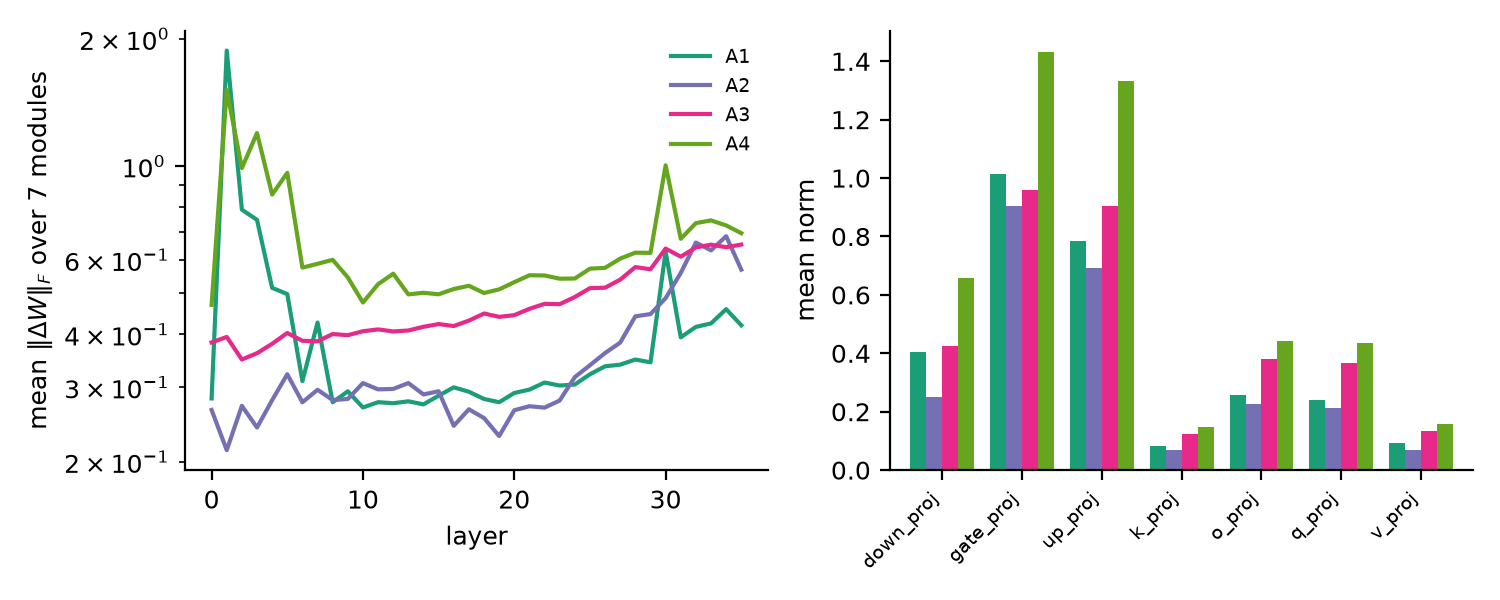
\includegraphics[width=.95\linewidth]{figs/fig_magnitude.png}
\caption{Left: mean $\|\Delta W\|_F$ per layer (log scale), averaged over the 7 modules. Right: mean norm per module type. Norms depend on matrix size, so compare within module type.}
\end{figure}
A4 modifies the weights most (mean 0.66) and A2 least (0.35); A1 0.41 and A3 0.47. MLP projections (gate, up) are altered far more than attention k/v. A1 and A4 have large outliers at layer 1 \texttt{gate\_proj} (10.28 and 6.61), and A4 at layer 3 \texttt{up\_proj} (4.58) and layer 30 \texttt{down\_proj} (3.31).

\subsection{Cosine similarity and sign conflict}
\begin{figure}[H]\centering
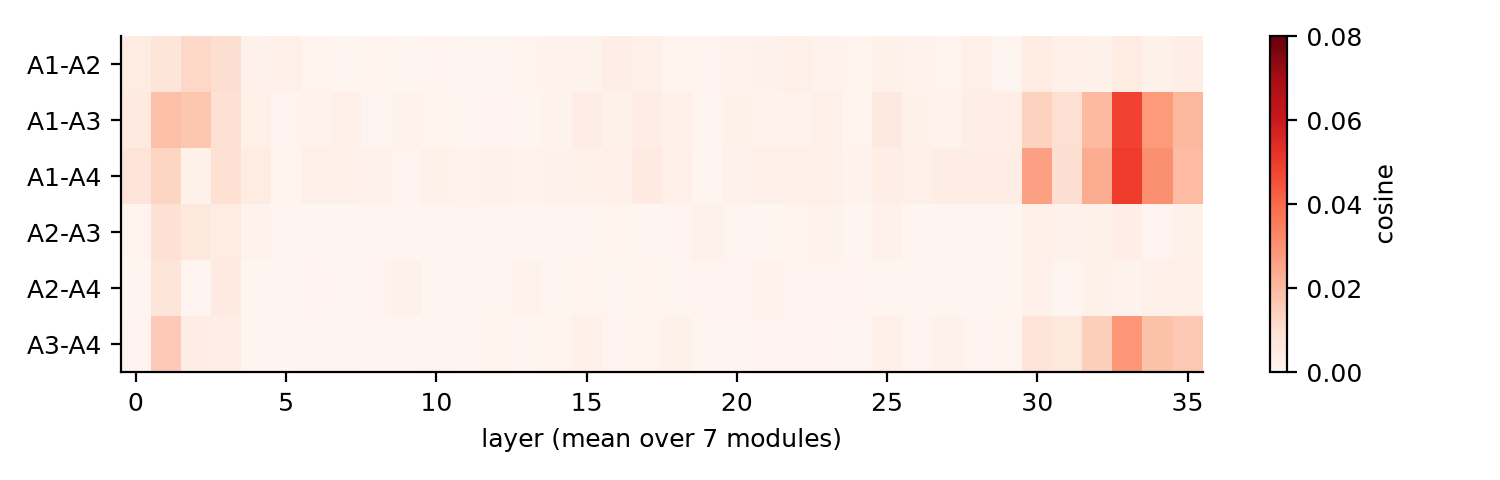
\includegraphics[width=.95\linewidth]{figs/fig_cos.png}
\caption{Pairwise cosine similarity by layer (mean over modules). Colour scale is 0--0.08; values this small are close to zero everywhere except layers 30--35.}
\end{figure}
\begin{figure}[H]\centering
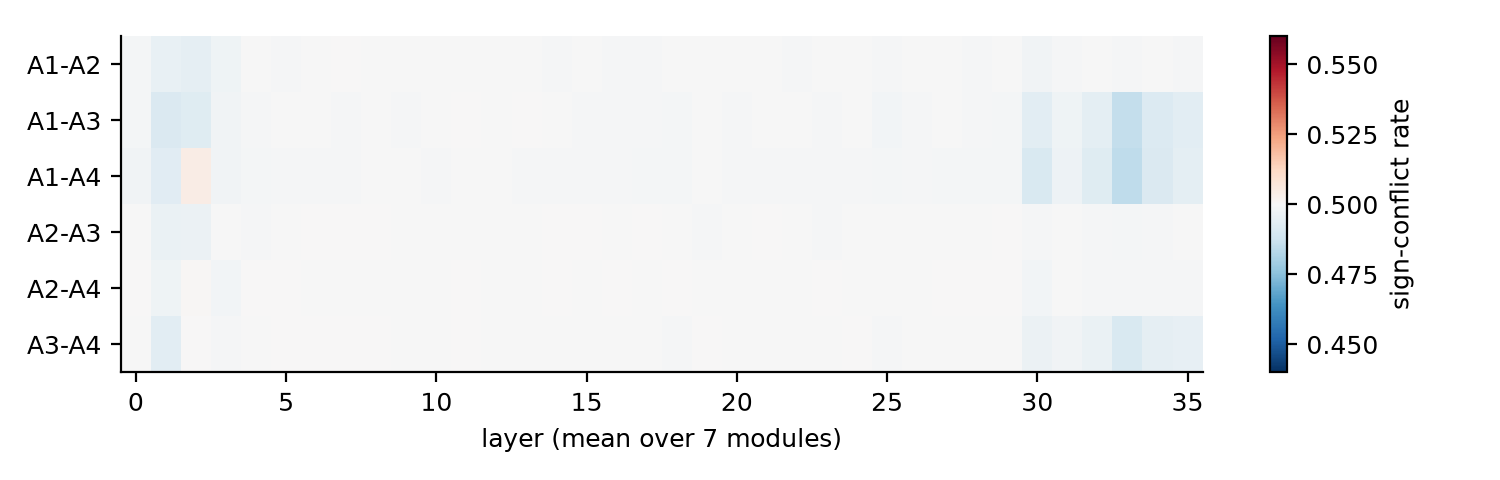
\includegraphics[width=.95\linewidth]{figs/fig_conf.png}
\caption{Pairwise sign-conflict rate by layer. 0.5 (white) is the rate expected for unrelated signs; blue is less conflict than chance.}
\end{figure}
\begin{figure}[H]\centering
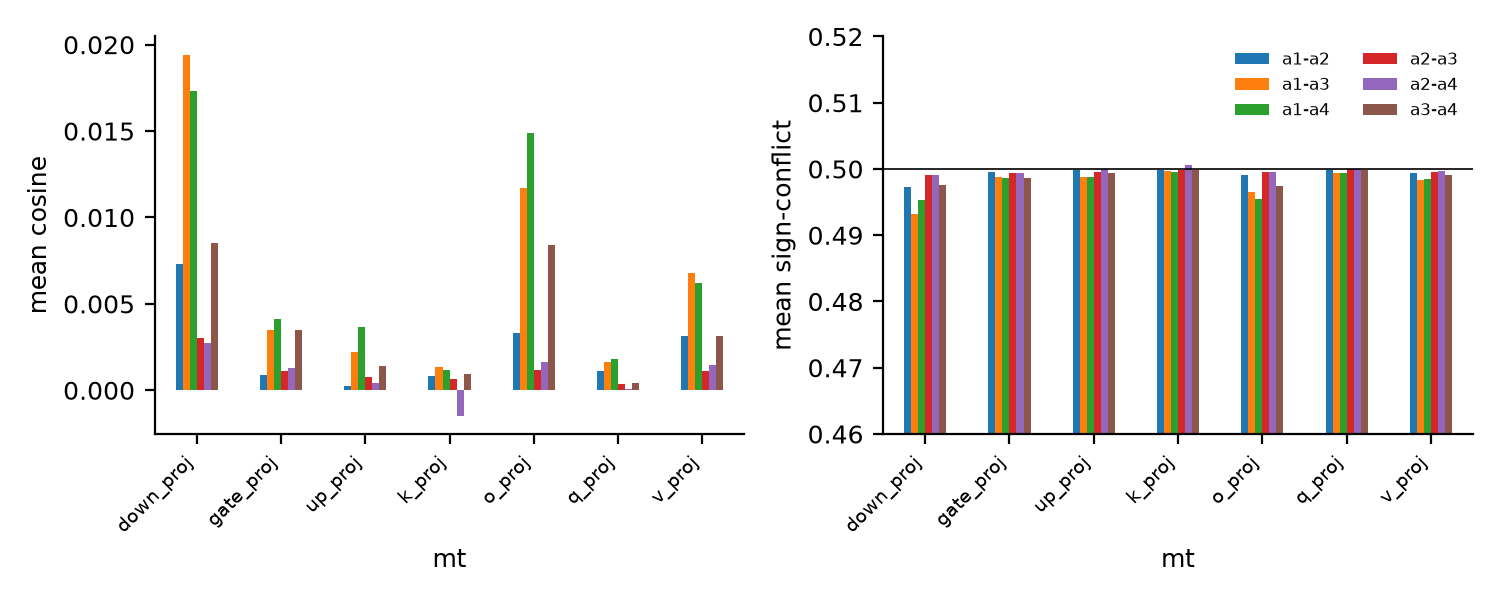
\includegraphics[width=.95\linewidth]{figs/fig_modtype.png}
\caption{Cosine and sign-conflict by module type, averaged over layers (right panel: the black line at 0.5 is chance).}
\end{figure}

\textbf{Findings.}
\begin{itemize}
\item Averaged over modules, every pair is almost exactly orthogonal and has about 50\% sign conflict. For two independent random matrices this is what one expects, so at the aggregate level these metrics \emph{do not} discriminate between pairs.
\item Structure is localised. The highest cosines are layer 33 \texttt{o\_proj} (A1--A4 0.211, A1--A3 0.168, A3--A4 0.127), layer 30 \texttt{down\_proj} (A1--A4 0.139) and layer 34 \texttt{down\_proj} (A1--A4 0.116). Layer 33 has the highest layer-mean cosine (0.023), followed by layers 34, 1 and 30. Sign conflict drops in the same places (down to 43.3\% for A1--A4 at layer 33 \texttt{o\_proj}), so the two metrics agree.
\item A1--A3 and A1--A4 are the most aligned pairs (9 and 8 modules with $|\cos|>0.05$); A3--A4 has 4, A1--A2 has 1, and A2--A3 and A2--A4 have none. A2 is the most distinct adapter.
\item By module type the mean cosine is largest for \texttt{down\_proj} (0.0097) and \texttt{o\_proj} (0.0069), both output-side projections.
\end{itemize}
\end{document}
